\documentclass[12pt,a4paper]{article}
\usepackage{amsmath,amssymb,makecell,fancyhdr,enumerate,arcs,physics,tasks,mathrsfs,graphics}
\usepackage{tikz,tikz-3dplot,tkz-euclide,tkz-tab,tabvar,pgfplots,esvect}
\usepackage[top=1.5cm, bottom=1.5cm, left=2cm, right=1.5cm]{geometry}
\usepackage[hidelinks,unicode]{hyperref}
\usepackage[utf8]{vietnam}
\usepackage[dethi]{ex_test}
\usetikzlibrary{shapes.geometric,shadings,calc,snakes,patterns,arrows,intersections,angles,backgrounds,quotes}
\usepgfplotslibrary{fillbetween}
\pgfplotsset{compat=newest}
\tikzset{point style/.append style={color=white}}
\def\vec{\overrightarrow}
\newcommand{\hoac}[1]{\left[\begin{aligned}#1\end{aligned}\right.}
\newcommand{\heva}[1]{\left\{\begin{aligned}#1\end{aligned}\right.}
\newcommand{\hetde}{\centerline{\rule[0.5ex]{2cm}{1pt} HẾT \rule[0.5ex]{2cm}{1pt}}}
\newcommand{\tentruong}{THPT Nguyễn Hữu Cảnh}
    \newcommand{\tengv}{Tổ Toán}
    \newcommand{\tenkythi}{Cộng Hoà Xã Hội Chủ Nghĩa Việt Nam}
    \newcommand{\tenmonthi}{Độc lập - tự do - hạnh phúc}
    \newcommand{\thoigian}{45}
    \newcommand{\tieude}[3]{
	\noindent
	%Trái
	\begin{minipage}[b]{7cm}
		\centerline{\textbf{\fontsize{13}{0}\selectfont \tentruong}}
		\centerline{\textbf{\fontsize{13}{0}\selectfont \tengv}}
		\centerline{------}
		\centerline{\textit{ }}
	\end{minipage}\hspace{1.5cm}
	%Phải
	\begin{minipage}[b]{9cm}
		\centerline{\textbf{\fontsize{13}{0}\selectfont \tenkythi}}
		\centerline{\textbf{\fontsize{13}{0}\selectfont \tenmonthi}}
		\centerline{\textit{\fontsize{12}{0}\selectfont ------ }}
		\centerline{\textit{\fontsize{12}{0}\selectfont  }}
	\end{minipage}
	\begin{minipage}[b]{13cm}
		\vspace*{.75cm}
		\textbf{Họ và tên: }{Nguyễn Văn Sang }\\
		% \textbf{Số Báo Danh: }{\tiny\dotfill}
	\end{minipage}
	\begin{minipage}[b]{8cm}
		% \hspace*{1cm}\fbox{\bf Mã đề thi #3}
	\end{minipage}
}
\newcommand{\chantrang}[2]{\rfoot{Trang \thepage $-$ Mã đề #2}}
\pagestyle{fancy}
\fancyhf{}
\renewcommand{\headrulewidth}{0pt}
\def\colorEX{}% màu phương án đúng
\renewtheorem{ex}{\color{blue!80!black}\textbf{Câu}}
    
    \newcommand{\made}{468}
    \begin{document}   
    \tieude{\pageref{\made}}{0}{\made}
    \chantrang{\pageref{\made}}{\made}
\begin{center}
    \textbf{Chuyên Đề Cá Nhân}\\
    \textbf{ĐỀ ÔN THI HỌC KỲ I - KHỐI 12}
\end{center}
\begin{center}
	\textbf{ĐỀ ÔN SỐ 1}
\end{center}
 \subsection*{PHẦN I. Câu trắc nghiệm nhiều phương án lựa chọn. Thí sinh trả lời từ câu 1 đến câu 13. Mỗi câu hỏi thí sinh chỉ chọn một phương án.}
    \setcounter{ex}{0}
    \Opensolutionfile{ans}[ans-phanI]
    \begin{ex}%[2D4N2-1]
	Cho $\displaystyle\int\limits_2^5 f\left( x \right)\mathrm{d}x=10$. Kết quả $\displaystyle\int\limits_5^2 \left[ 2-4f\left( x \right) \right]\mathrm{d}x$ bằng
	\choice
{$40$}
{\True $34$}
{$32$}
{$36$}
	\loigiai{
		Ta có
		\allowdisplaybreaks
		\begin{eqnarray*}
			\displaystyle\int\limits_5^2 \left[ 2-4f\left( x \right) \right]\mathrm{d}x &=& 2\displaystyle\int\limits_5^2 \mathrm{d}x-4\displaystyle\int\limits_5^2 f\left( x \right)\mathrm{d}x\\
			&=& -2x \Big|_2^5+4\displaystyle\int\limits_2^5 f\left( x \right)\mathrm{d}x\\
			&=& -2\cdot\left( 5-2 \right)+4\cdot 10=34.
		\end{eqnarray*}
	}
\end{ex}
\begin{ex}%[2H5N2-2]
	Trong không gian $Oxyz$, cho đường thẳng $d\colon \dfrac{x-2}{1}=\dfrac{y-1}{2}=\dfrac{z+1}{2}$ nhận véc-tơ $\overrightarrow{u}=(a;2;b)$ làm véc-tơ chỉ phương. Khi đó $a+b$ bằng
	\choice
{$-5$}
{\True $3$}
{$-3$}
{$5$}
	\loigiai{
		Đường thẳng $d$ có một véc-tơ chỉ phương là $\overrightarrow{u}_d=(1;2;2) \Rightarrow \heva{&a=1\\ &b=2} \Rightarrow a+b=3$.
	}
\end{ex}
\begin{ex}%[2H5H2-7]
	Trong không gian $Oxyz$, cho hai đường thẳng $d_1 \colon \dfrac{x-1}{2}=\dfrac{y+2}{-1}=\dfrac{z-4}{2}$ và \\ $d_2\colon \heva{&x=3+t \\& y=-t \\& z=4}$. Tính góc giữa $d_1$ và $d_2$.
	\choice
{$90^\circ$}
{\True $45^\circ$}
{$30^\circ$}
{$60^\circ$}
	\loigiai{
		Gọi $\varphi$ là góc giữa đường thẳng $d_1$ và $d_2$.\\
		Đường thẳng $d_1$ có véc-tơ chỉ phương $\vec{a}_1=(2;-1;2).$\\
		Đường thẳng $d_2$ có véc-tơ chỉ phương $\vec{a}_2=(1;-1;0).$\\
		Ta có $\cos \varphi=\dfrac{\left| \overrightarrow{a}_{d_1}\cdot\overrightarrow{a}_{d_2} \right|}{\left| \overrightarrow{a}_{d_1} \right|\cdot\left| \overrightarrow{a}_{d_2} \right|}=\dfrac{3}{3\sqrt{2}} \Rightarrow \varphi = 45^\circ$.
	}
\end{ex}
\begin{ex}%[2H5H2-7]
	Trong không gian với hệ tọa độ $Oxyz$, cho mặt phẳng $(\alpha)\colon x-y+2z+1=0$ và đường thẳng $\Delta\colon \dfrac{x}{1}=\dfrac{y}{2}=\dfrac{z-1}{-1}$. Góc giữa $\Delta$ và $(\alpha)$ bằng
	\choice
{$60^\circ$}
{\True $30^\circ$}
{$120^\circ$}
{$45^\circ$}
	\loigiai{
		Mặt phẳng $(\alpha)$ có véc-tơ pháp tuyến $\vec{n}_{\alpha}=(1;-1;2)$.\\
		Đường thẳng $\Delta$ có véc-tơ chỉ phương $\vec{u}_\Delta=(1;2;-1)$.\\
		Gọi $\varphi$ là góc giữa đường thẳng $\Delta$ và mặt phẳng $(\alpha)$.\\
		Ta có $\sin\varphi=\dfrac{|1-2-2|}{\sqrt{6}\cdot \sqrt{6}}=\dfrac{1}{2}\Rightarrow\varphi=30^\circ.$
	}
\end{ex}
\begin{ex}%[2H5H3-3]
	Trong không gian $O x y z$, phương trình nào dưới đây là phương trình mặt cầu tâm $I(1 ; 0 ;-2)$, bán kính $r=4$?
	\choice
{$(x-1)^{2}+y^{2}+(z+2)^{2}=4$}
{$(x+1)^{2}+y^{2}+(z-2)^{2}=16$}
{\True $(x-1)^{2}+y^{2}+(z+2)^{2}=16$}
{$(x+1)^{2}+y^{2}+(z-2)^{2}=4$}
	\loigiai{
		Phương trình mặt cầu là $(x-1)^{2}+y^{2}+(z+2)^{2}=16$.
	}
\end{ex}
\begin{ex}%[2H5H3-3]
	Trong không gian $O x y z$, mặt cầu $(S)$ có tâm có tâm $I(1 ;-3 ; 2)$ và đi qua điểm $A(5 ;-1 ; 4)$ là
	\choice
{$(x-1)^{2}+(y+3)^{2}+(z-2)^{2}=\sqrt{24}$}
{\True $(x-1)^{2}+(y+3)^{2}+(z-2)^{2}=24$}
{$(x+1)^{2}+(y-3)^{2}+(z+2)^{2}=\sqrt{24}$}
{$(x+1)^{2}+(y-3)^{2}+(z+2)^{2}=24$}
	\loigiai{
		Mặt cầu có bán kính $R=IA=\sqrt{(5-1)^2+(-1+3)^2+(4-2)^2}=2\sqrt{6}$.\\
		Phương trình mặt cầu là $(x-1)^{2}+(y+3)^{2}+(z-2)^{2}=24$.
	}
\end{ex}
\begin{ex}%[2H5H3-3]
	Trong không gian $O x y z$, cho mặt cầu $(S)$ có tâm $I(-1 ; 4 ; 2)$ và thể tích bằng $\dfrac{256 \pi}{3}$. Phương trình của $(S)$ là
	\choice
{\True $(x+1)^{2}+(y-4)^{2}+(z-2)^{2}=16$}
{$(x-1)^{2}+(y+4)^{2}+(z+2)^{2}=4$}
{$(x-1)^{2}+(y+4)^{2}+(z+2)^{2}=4$}
{$(x+1)^{2}+(y-4)^{2}+(z-2)^{2}=4$}
	\loigiai{
		Mặt cầu có  thể tích bằng $\dfrac{256 \pi}{3}$ nên $\dfrac{4 \pi R^3}{3}=\dfrac{256 \pi}{3} \Leftrightarrow R^3=64 \Leftrightarrow R=4$.\\
		Phương trình mặt cầu là $(x+1)^{2}+(y-4)^{2}+(z-2)^{2}=16$.
	}
\end{ex}
\begin{ex}%[2H5H3-3]
	Trong không gian với hệ toạ độ $Oxyz$, cho mặt phẳng $(P) \colon 6x+3y-2z+24=0$ và điểm $I(2;5;1)$. Mặt cầu tâm $I$ và tiếp xúc với mặt phẳng $(P)$ có phương trình là
	\choice
{$(x+2)^2+(y+5)^2+(z+1)^2=7$}
{$(x+2)^2+(y+5)^2+(z+1)^2=49$}
{$(x-2)^2+(y-5)^2+(z-1)^2=7$}
{\True $(x-2)^2+(y-5)^2+(z-1)^2=49$}
	\loigiai{
		Mặt cầu tâm $I$ và tiếp xúc với mặt phẳng $(P)$ nên
		$$R= \mathrm{d}\left(I,(P)\right)= \dfrac{\left|6\cdot 2+3\cdot 5-2\cdot 1+24\right|}{\sqrt{6^2+3^2+(-2)^2}}=7.$$
		Phương trình mặt cầu là $(x-2)^2+(y-5)^2+(z-1)^2=49$.
	}
\end{ex}
\begin{ex}%[2D6H1-2]
	Một hộp có $8$ viên bi đỏ và $7$ viên bị xanh, các viên bi có cùng kích thước và khối lượng. Bạn Hoa lấy một viên bi trong hộp, không trả lại. Sau đó bạn Hồng lấy một viên bi trong hộp đó. Tính xác suất để bạn Hồng lấy được viên bi đỏ nếu biết rằng bạn Hoa lấy được viên bi đỏ.
	\choice
{\True $\dfrac{1}{2}$}
{$\dfrac{4}{7}$}
{$\dfrac{8}{15}$}
{$\dfrac{7}{15}$}
	\loigiai{
		Gọi $A$ là biến cố \lq\lq Hồng lấy được bi đỏ\rq\rq\, và $B$ là biến cố \lq\lq Hoa lấy được bi đỏ\rq\rq.\\
		Hoa có $15$ cách chọn, Hồng có $14$ cách chọn một viên bi. Do đó $n\left(\Omega\right)= 15\cdot 14$.\\
		Hoa có $8$ cách chọn một viên bi đỏ, Hồng có $14$ cách chọn một trong các viên bi còn lại.\\
		Do đó $n \left(B\right)=8\cdot 14$ và $\mathrm{P}\left(B\right)= \dfrac{n\left(B\right)}{n\left(\Omega\right)}$.\\
		Hoa có $8$ cách chọn một viên bi đỏ, Hồng có $7$ cách chọn một viên bi đỏ còn lại.\\
		Do đó $n \left(AB\right)=8\cdot 7$ và $\mathrm{P}\left(AB\right)= \dfrac{n\left(AB\right)}{n\left(\Omega\right)}$.\\
		Vậy $\mathrm{P}\left(A|B\right)= \dfrac{\mathrm{P}\left(AB\right)}{\mathrm{P}\left(B\right)} = \dfrac{n\left(AB\right)}{n\left(B\right)}= \dfrac{8\cdot 7}{8\cdot 14}= \dfrac{1}{2}$.
	}
\end{ex}
\begin{ex}%[2D6H1-2]
	Cho các biến cố $A$ và $B$ thỏa mãn $\mathrm{P}\left(A\right)=0{,}3$; $\mathrm{P}\left(B\right)=0{,}5$; $\mathrm{P}\left(B|A\right)=0{,}7$. Tính $\mathrm{P}\left(A|B\right)$.
	\choice
{$\dfrac{2}{5}$}
{\True $\dfrac{21}{50}$}
{$\dfrac{19}{50}$}
{$\dfrac{11}{25}$}
	\loigiai{
		Ta có $\mathrm{P}\left(AB\right)=\mathrm{P}\left(B|A\right)\cdot \mathrm{P}\left(A\right) = 0{,}7\cdot 0{,}3=0{,}21$.\\
		Lại có $\mathrm{P}\left(A|B\right)= \dfrac{\mathrm{P}\left(AB\right)}{\mathrm{P}\left(B\right)}= \dfrac{0{,}21}{0{,}5}= \dfrac{21}{50}$.
	}
\end{ex}
\begin{ex}%[2D6H2-2]
	Người ta khảo sát khả năng chơi nhạc cụ của một nhóm học sinh tại trường X. Nhóm này có $60\%$ học sinh là nam. Kết quả khảo sát cho thấy có $20\%$ học sinh nam và $15\%$ học sinh nữ biết chơi ít nhất một nhạc cụ. Chọn ngẫu nhiên một học sinh trong nhóm này. Tính xác suất để chọn được học sinh biết chơi ít nhất một nhạc cụ.
	\choice
{$19\%$}
{\True $18\%$}
{$16\%$}
{$17\%$}
	\loigiai{
		Xét phép thử chọn ngẫu nhiên một học sinh trong nhóm và xét
		\begin{itemize}
			\item $A$ là biến cố \lq\lq Chọn được một học sinh biết chơi ít nhất một nhạc cụ\rq\rq;
			\item $B$ là biến cố \lq\lq Chọn được một học sinh nam\rq\rq;
			\item $\overline{B}$ là biến cố \lq\lq Chọn được một học sinh nữ\rq\rq.
		\end{itemize}
		Theo đề bài
		$$\mathrm{P}(B) = 60\% = 0{,}6;\quad \mathrm{P}(\overline{B}) = 1 - 0{,}6 = 0{,}4;$$
		$$\mathrm{P}(A|B) = 20\% = 0{,}2;\quad \mathrm{P}(A|\overline{B}) = 15\% = 0{,}15.$$
		Áp dụng công thức xác suất toàn phần, ta có
		$$\mathrm{P}(A) = \mathrm{P}(B)\cdot \mathrm{P}(A|B) + \mathrm{P}(\overline{B})\cdot \mathrm{P}(A|\overline{B}) = 0{,}6\cdot 0{,}2 + 0{,}4\cdot 0{,}15 = 0{,}18.$$
		Vậy xác suất để chọn được một học sinh biết chơi nhạc cụ là $0{,}18$ hay $18\%$.
	}
\end{ex}
\begin{ex}%[2D6H2-3]
	Có hai hộp đựng các viên bi cùng kích thước và khối lượng. Hộp thứ nhất chứa $5$ viên bi đỏ và $5$ viên bi xanh, hộp thứ hai chứa $6$ viên bi đỏ và $4$ viên bi xanh. Lấy ngẫu nhiên một viên bi từ hộp thứ nhất chuyển sang hộp thứ hai, sau đó lấy ra ngẫu nhiên một viên bi từ hộp thứ hai (giả sử viên bi được lấy ra từ hộp thứ hai là bi đỏ). Tính xác suất viên bi đỏ đó là của hộp thứ nhất.
	\choice
{\True $\dfrac{25}{58}$}
{$\dfrac{29}{55}$}
{$\dfrac{1}{2}$}
{$\dfrac{5}{11}$}
	\loigiai{
		Gọi $A$ là biến cố \lq\lq viên bi được chọn từ hộp thứ nhất\rq\rq.\\
		$B$ là biến cố \lq\lq viên bi đỏ được lấy ra từ hộp thứ hai\rq\rq.\\ $\overline{A}$ là biến cố \lq\lq viên bi được từ hộp thứ hai\rq\rq.\\
		Ta có $\mathrm{P}(A)=\dfrac{1}{2}$ và $\mathrm{P}\left(\overline{A}\right)=1-\dfrac{1}{2}=\dfrac{1}{2}$.\\
		Xác suất viên bi đỏ được lấy từ hộp thứ hai khi đã chọn từ hộp thứ nhất
		$$\mathrm{P}(B|A)=\dfrac{\mathrm{C}_5^1}{\mathrm{C}_{11}^1}=\dfrac{5}{11}.$$
		Xác suất viên bi đỏ được lấy từ hộp thứ hai khi không chọn từ hộp thứ nhất
		$$\mathrm{P}\left(B|\overline{A}\right)=\dfrac{\mathrm{C}_6^1}{\mathrm{C}_{10}^1}=\dfrac{6}{10}=\dfrac{3}{5}.$$
		Ta có $\mathrm{P}(B)=\mathrm{P} (B|A)\cdot \mathrm{P} (A)+\mathrm{P} \left(B|\overline{A}\right)\cdot \mathrm{P}\left(\overline{A}\right)=\dfrac{5}{11}\cdot \dfrac{1}{2}+\dfrac{3}{5}\cdot \dfrac{1}{2}=\dfrac{29}{55}$.\\
		Theo công thức Bayes, ta có $$\mathrm{P}(A|B)=\dfrac{\mathrm{P}(B|A)\cdot\mathrm{P}(A)}{\mathrm{P}(B)}=\dfrac{\dfrac{5}{11}\cdot \dfrac{1}{2}}{\dfrac{29}{55}}=\dfrac{25}{58}.$$
	}
\end{ex}
    \Closesolutionfile{ans}
    
    \subsection*{PHẦN II. Câu trắc nghiệm đúng sai. Thí sinh trả lời từ câu 1 đến câu 4. Trong mỗi ý a), b), c), d) ở mỗi câu, thí sinh chọn đúng hoặc sai.}
    \setcounter{ex}{0}
    \Opensolutionfile{ans}[ans-phanII]
    \begin{ex}
	Trong không gian với hệ tọa độ $Oxyz$, cho mặt cầu $(S)\colon x^2+y^2+z^2-4x+2y+2z-10=0$ và mặt phẳng $(P)\colon x+2y-2z+10=0$
	\choiceTF
{\True $(P)$ tiếp xúc với $(S)$}
{\True Bán kính của mặt cầu $(S)$ là $R=4$}
{Véc-tơ pháp tuyến của $(P)$ là $\overrightarrow{n}=\left(1;2;2 \right) $}
{\True Mặt cầu $(S)$ có tâm $I\left(2;-1;-1\right)$}
	\loigiai{
		\begin{itemchoice}
			\itemch Đúng. Ta có \allowdisplaybreaks \begin{eqnarray*}
				&&x^2+y^2+z^2-4x+2y+2z-10=0\\
				&&(x^2-4x+4)+(y^2+2y+1)+(z^2+2z+1)=16\\
				&& (x-2)^2+(y+1)^2+(z+1)^2=16
			\end{eqnarray*}
		Vậy mặt cầu $(S)$ có tâm $I\left(2;-1;-1\right)$.
			\itemch Đúng. Ta có $(S)\colon (x-2)^2+(y+1)^2+(z+1)^2=16=4^2$ nên mặt cầu $(S)$ có bán kính $R=4$.
			\itemch Sai. Ta có $(P)\colon x+2y-2z+10=0$ nên véc-tơ pháp tuyến của $(P)$ là $\overrightarrow{n}=\left(1;2;-2\right)$
			\itemch Đúng.  Khoảng cách từ tâm $I$ đến mặt phẳng $(P)$ là \begin{eqnarray*}
				\mathrm{\,d}\left(I,\left(P \right)  \right)=\dfrac{\left|2+2\cdot\left(-1\right)-2\cdot\left(-1 \right)+10   \right| }{\sqrt{1^2+2^2+\left(-2\right)^2 }}=\dfrac{12}{3}=4
			\end{eqnarray*}	
		Ta thấy $	\mathrm{\,d}\left(I,\left(P \right)\right) =R$ nên $(P)$ tiếp xúc với $(S)$.
		\end{itemchoice}
	}
\end{ex}
\begin{ex}
	Vào mỗi buổi sáng ở tuyến phố H, xác suất xảy ra
	tắc đường khi trời mưa và không mưa lần lượt là $0{,}7$
	và $0{,}2$. Xác suất có mưa vào một buổi sáng là $0{,}1$.
	\choiceTF
{\True 	Xác suất không có mưa vào một buổi sáng $0{,}9$}
{Xác suất xảy ra tắc đường khi trời không mưa là $0{,}7$}
{\True Xác suất để sáng đó tuyến phố H bị tắc đường là $0{,}25$}
{Xác suất xảy ra tắc đường khi trời mưa  là $0{,}2$}
	\loigiai{
		\begin{itemchoice}
			\itemch Sai. Gọi $ A $ là biến cố \lq\lq Trời mưa vào một buổi sáng\rq\rq  và $ B $ là biến cố \lq\lq Tuyến phố H tắc đường\rq\rq.
			Do xác suất xảy ra tắc đường khi trời mưa  là $ 0{,}7 $ nên $ \mathrm{P}(B|A)=0{,}7 $.
			\itemch Sai. 
			Do xác suất xảy ra tắc đường khi trời không mưa là $ 0{,}2 $ nên $ \mathrm{P}(B|\overline{A}) =0{,}2$.
			\itemch Đúng. 
			Do xác suất có mưa vào một buổi sáng là $ 0{,}1 $ nên $ \mathrm{P}(A)=0{,}1 $ và $ \mathrm{P}(\overline{A})=0{,}9 $.
			\itemch Đúng.
			Áp dụng công thức xác suất toàn phần, ta có xác suất để sáng đó tuyến phố H bị tắc đường là\allowdisplaybreaks
			\begin{eqnarray*}
				 \mathrm{P}(B)=\mathrm{P}(A)\mathrm{P}(B|A)+\mathrm{P}(\overline{A})\mathrm{P}(B|\overline{A})=0{,}1 \cdot 0{,}7+0{,}9 \cdot 0{,}2= 0{,}25.
			\end{eqnarray*}
		\end{itemchoice}
	}
\end{ex}
\begin{ex}
	Một nhóm $5$ học sinh nam và $4$ học sinh nữ tham gia lao động trên sân trường. Cô giáo chọn ngẫu nhiên đồng thời $2$ bạn trong nhóm đi tưới cây. 
	\choiceTF
{Số phần tử của biến cố có ít nhất một bạn nam được chọn là $10$}
{Xác suất để hai bạn được chọn có cùng giới tính nam là $\dfrac{1}{3}$}
{\True Xác suất để trong hai bạn được chọn có ít nhất $1$ bạn nam được chọn là $\dfrac{15}{36}$}
{\True Số phần tử của không gian mẫu là $n(\Omega)=\mathrm{C}^2_9=36$}
	\loigiai{
		\begin{itemchoice}
			\itemch Đúng. Số phần tử của không gian mẫu là $n(\Omega)=\mathrm{C}^2_9=36$.
			\itemch Sai. Gọi $A$ là biến cố \lq\lq Hai bạn được chọn có cùng giới tính\rq\rq.\\
			B là biến cố \lq\lq Có ít nhất một bạn nam được chọn\rq\rq.\\
			Ta có $n(B)=\mathrm{C}^2_5+\mathrm{C}^1_5=15$.
			\itemch Đúng. \\Gọi A là biến cố \lq\lq Hai bạn được chọn có cùng giới tính\rq\rq.\\
			B là biến cố \lq\lq Có ít nhất một bạn nam được chọn\rq\rq.\\
			Ta có $n(B)=\mathrm{C}^2_5+\mathrm{C}^1_5=15$ suy ra $\mathrm{P}(B)=\dfrac{15}{36}$.
			\itemch Sai. \\	Ta có $n(AB)=C^2_5=10$ suy ra $\mathrm{P}(AB)=\dfrac{10}{36}$.\\
			Vậy $\mathrm{P}(A|B)=\dfrac{\mathrm{P}(AB)}{\mathrm{P}(B)}=\dfrac{10}{15}=\dfrac{2}{3}$.
		\end{itemchoice}
	}
\end{ex}
\begin{ex}
	Trong không gian với hệ toạ độ $Oxyz$ cho đường thẳng $d\colon\heva{&x=1-t\\&y=2+2t\\&z=3+t}$, và mặt phẳng $(P)\colon x-y+3=0$. 
	\choiceTF
{Góc giữa đường thẳng $d$ và mặt phẳng $(P)$ bằng $30^{\circ}$}
{Mặt phẳng $(P)$ có véc-tơ pháp tuyến là $\overrightarrow{n}=\left(1;-1;3 \right) $}
{\True Điểm $A(-1;-2;0)\in \left(P\right) $}
{\True Đường thẳng $d$ có véc-tơ chỉ phương là $\overrightarrow{u}=\left(-1;2;1 \right) $}
	\loigiai{
		\begin{itemchoice}
			\itemch Đúng. Đường thẳng $d\colon\heva{&x=1-t\\&y=2+2t\\&z=3+t}$ có véc-tơ chỉ phương là $\overrightarrow{u}=\left(-1;2;1 \right)$.
			\itemch Sai. Mặt phẳng $(P)\colon x-y+3=0$ có véc-tơ pháp tuyến là $\overrightarrow{n}=\left(1;-1;0 \right)$.
			\itemch Đúng. Thay $A(-1;-2;0)\in \left(P\right) $ vào mặt phẳng $(P)\colon x-y+3=0$ thấy thoả mãn nên $A(-1;-2;0)\in \left(P\right) $.
			\itemch Sai. Gọi $\alpha$ là góc giữa đường thẳng $d$ và mặt phẳng $(P)$. Khi đó, ta có\begin{eqnarray*}
				\sin \alpha=\dfrac{\left|\overrightarrow{u}\cdot\overrightarrow{n} \right| }{\left|\overrightarrow{u} \right|\cdot\left|\overrightarrow{n} \right|}=\dfrac{\left|-1\cdot1+2\cdot(-1)+1\cdot0 \right| }{\sqrt{\left(-1\right)^2+2^2+1^2 }\cdot\sqrt{1^2+\left(-1\right)^2 +0^2}}=\dfrac{\sqrt{3}}{2} 
			\end{eqnarray*} 
		Do đó, $\alpha=60^{\circ}$.
		\end{itemchoice}
	}
\end{ex}
    \Closesolutionfile{ans}
    
    \subsection*{PHẦN III. Câu hỏi trả lời ngắn. Thí sinh trả lời từ câu 1 đến câu 6.}
    \setcounter{ex}{0}
    \Opensolutionfile{ans}[ans-phanIII]
    \begin{ex}%[2H5H1-3]
	Trong không gian $O x y z$, phương trình mặt phẳng đi qua $M(3 ;-1 ; 2)$, $N(4 ;-1 ;-1)$, $\mathrm{P}(2 ; 0 ; 2)$ có dạng $3x+By+Cz+D=0$. Tính $B^2+C^2+D^2$.
	\shortans{$74$}
	\loigiai{
		Ta có $\overrightarrow{MN}=(1;0;-3)$, $\overrightarrow{MP}=(-1;1;0)$.\\
		Mặt phẳng đi qua điểm $M(3 ;-1 ; 2)$ và có véc-tơ pháp tuyến $\vec{n}=\left[\overrightarrow{MN},\overrightarrow{MP}\right]=(3;3;1)$ có phương trình là
		$$3(x-3)+3(y+1)+1(z-2)=0\Leftrightarrow 3x+3y+z-8=0.$$
		Vậy $B=3$, $C=1$, $D=-8$ suy ra $B^2+C^2+D^2=3^2+1^2+(-8)^2=74$.
	}
\end{ex}
\begin{ex}%[2H5V2-7]
	Trong không gian với hệ tọa độ $Oxyz$, cho đường thẳng $d\colon \dfrac{x+1}{2}= \dfrac{y+1}{1}= \dfrac{z-3}{1}$ và mặt phẳng $(P)\colon x+2y-z+5=0$. Mặt phẳng $(Q)$ chứa đường thẳng $d$ và tạo với $(P)$ một góc nhỏ nhất có phương trình dạng $Ax+By-z+D=0$. Tính $A^2+B^2+D^2$.
	\shortans{$17$}
	\loigiai{
		Ta có $M(-1;-1;3)\in d$;  $N(1;0;4)\in d$.\\
		Phương trình mặt phẳng $(Q)$ có dạng $Ax+By-z+D=0.$\\
		Vì $M, N\in d$ nên
		\[\heva{&-A-B-3+D=0\\& A-4+D=0}\Leftrightarrow \heva{&B=-2A+1\\&D=-A+4.}\]
		Do đó $\vec{n}_Q=(A; B; -1)$.\\
		Ta có $\vec{n}_P=(1;2;-1)$.\\
		Gọi $\varphi$ là góc tạo bởi mặt phẳng $(P)$ và mặt phẳng $(Q)$.\\
		\[\cos\varphi=\dfrac{|A+2B+1|}{\sqrt{A^2+B^2+(-1)^2}\cdot \sqrt{6}}=\dfrac{3}{\sqrt{6}}\cdot\dfrac{|A-1|}{\sqrt{5A^2-4A+2}}.\]
		Trường hợp $A-1=0 \Leftrightarrow A=1$, ta có $\varphi =90^\circ$ là góc lớn nhất trong các góc có thể giữa hai mặt phẳng $(P)$ và $(Q)$, do đó loại trường hợp này.\\
		Trường hợp $A-1
eq 0 \Leftrightarrow A 
e 1$, ta có
		\[\cos\varphi=\dfrac{3}{\sqrt{6}}\cdot\sqrt{\dfrac{(A-1)^2}{2(A-1)^2+3A^2}}=\dfrac{3}{\sqrt{6}}\cdot \sqrt{\dfrac{1}{2+3\cdot\left(\dfrac{A}{A-1} \right)^2 }}\le \dfrac{3}{\sqrt{6}}\cdot \sqrt{\dfrac{1}{2}}=\dfrac{\sqrt{3}}{2},\]
		Suy ta $\varphi\ge 30^\circ$.\\
		Dấu \lq\lq $=$\rq\rq\, xảy ra khi $A=0$. Khi đó $B=1$ và $D=-A+4=4$.\\
		Do đó mặt phẳng $(Q)$ chứa đường thẳng $d$ và tạo với $(P)$ một góc nhỏ nhất có phương trình là
		\[y-z+4=0.\]
		Vậy $A=0$; $B=1$; $D=4$ suy ra $A^2+B^2+D^2=0^2+1^2+4^2=17$.
	}
\end{ex}
\begin{ex}%[2H5H3-2]
	Trong không gian $O x y z$, cho điểm $I(-4 ;-2 ; 3)$. Tính bán kính của mặt cầu $(S)$ có tâm $I$ và tiếp xúc với trục tung $Oy$.
	\shortans[]{$5$}
	\loigiai{
		Bán kính $R=\mathrm{d}(I,Oy)=\sqrt{(-4)^2+3^2}=5$.
	}
\end{ex}
\begin{ex}%[2H5V3-3]
	Trong không gian với hệ tọa độ $Oxyz$, phương trình mặt cầu đi qua bốn điểm $M(1; 0; 1)$, $N(1; 0; 0)$, $P(2 ; 1 ; 0)$ và $Q(1; 1; 1)$ có dạng $(S)\colon x^2+y^2+z^2-2ax-2by-2cz+d=0$. Tính $a+b+c+d$.
	\shortans{$4{,}5$}
	\loigiai{
		Ta có
		\begin{itemize}
			\item $M(1;0;1)\in(S)\Leftrightarrow 1^2+0^2+1^2-2a\cdot 1-2b\cdot 0-2c\cdot 1 +d=0\Leftrightarrow -2a-2c+d=-2$. \quad(1)
			\item $N(1;0;0)\in(S)\Leftrightarrow 1^2+0^2+0^2-2a\cdot 1-2b\cdot 0-2c\cdot 0 +d=0\Leftrightarrow -2a+d=-1$. \quad(2)
			\item $\mathrm{P}(2;1;0)\in(S)\Leftrightarrow 2^2+1^2+0^2-2a\cdot 2-2b\cdot 1-2c\cdot 0 +d=0\Leftrightarrow -4a-2b+d=-5$. \quad(3)
			\item $Q(1;1;1)\in(S)\Leftrightarrow 1^2+1^2+1^2-2a\cdot 1-2b\cdot 1-2c\cdot 1 +d=0\Leftrightarrow -2a-2b-2c+d=-3$. \quad(4)
		\end{itemize}
		Từ (1),(2),(3),(4) ta có hệ
		\allowdisplaybreaks
		\begin{eqnarray*}
			\heva{&-2a-2c+d=-2\\&-2a+d=-1\\&-4a-2b+d=-5\\&-2a-2b-2c+d=-3} &\Leftrightarrow& \heva{&-2a-2c-1+2a=-2\\&d=-1+2a\\&-4a-2b-1+2a=-5\\&-2a-2b-2c-1+2a=-3}\\
			&\Leftrightarrow& \heva{&d=-1+2a\\&-2c=-1\\&-2a-2b=-4\\&-2b-2c=-2}\\
			&\Leftrightarrow& \heva{&a=\dfrac{3}{2}\\&b=\dfrac{1}{2}\\&c=\dfrac{1}{2}\\&d=2.}
		\end{eqnarray*}
		Vậy $a+b+c+d=\dfrac{3}{2}+ \dfrac{1}{2}+ \dfrac{1}{2}+2=4{,}5$.
	}
\end{ex}
\begin{ex}%[2D6V2-2]
	Một nghiên cứu đã chỉ ra rằng tỉ lệ người bị lao phổi trong nhóm $X$ những người mắc phải hội chứng suy giảm miễn dịch $H$ là $15{,}2 \%$. Kết quả nghiên cứu về một số triệu chứng lâm sàng như có ho trong vòng bốn tuần, hoặc có bị sốt trong vòng bốn tuần, hoặc ra mồ hôi ban đêm từ ba tuần trở lên của nhóm $X$ cho thấy.
	\begin{itemize}
		\item Trong số những người mắc bệnh lao phổi, có $93{,}2 \%$ trường hợp có ít nhất một triệu chứng;
		\item Trong số những người không mắc bệnh lao phổi, có $35{,}8 \%$ trường hợp không có triệu chứng nào.
	\end{itemize}
	Nếu bác sĩ gặp một bệnh nhân thuộc nhóm $X$ và bệnh nhân đó có ít nhất một triệu chứng trên thì xác suất bệnh nhân này mắc bệnh lao phổi là bao nhiêu? (kết quả làm tròn đến phần trăm)
	\shortans[]{$0,21$}
	\loigiai{
		Gọi $A$ là biến cố \lq\lq Người bị lao phổi\rq\rq.\\
		$\overline{A}$ là biến cố \lq\lq Người không mắc lao phổi\rq\rq.\\
		$B$ là biến cố \lq\lq Những người có ít nhất một triệu chứng\rq\rq.\\
		$\overline{B}$ là biến cố \lq\lq Những người không có triệu chứng\rq\rq.\\
		Ta có $\mathrm{P}(A)=0{,}152$. \\
		Khi đó, xác suất những người không mắc lao phổi là $$\mathrm{P}\left(\overline{A}\right)=1-0{,}152=0{,}848.$$
		Ta có xác suất những người có ít một triệu chứng trong những người mắc lao phổi là $$\mathrm{P}\left(B|A\right)=0{,}932.$$
		Khi đó, xác suất những người không có triệu chứng trong những người mắc lao phổi là  $$\mathrm{P}\left(\overline{B}|A\right)=1-0{,}932=0{,}068.$$
		Mặt khác, ta có xác suất những người không có triệu chứng  $$\mathrm{P}\left(\overline{B}|\overline{A}\right)=0{,}358.$$
		Khi đó, xác suất những người có ít nhất một triệu chứng trong những người không mắc bệnh lao phổi là $$\mathrm{P}\left(B|\overline{A}\right)=1-0{,}358=0{,}642.$$
		Ta có $\mathrm{P}(B)=\mathrm{P}\left(B|A\right)\cdot \mathrm{P}(A)+\mathrm{P}\left(B|\overline{A}\right)\cdot \mathrm{P}\left(\overline{A}\right)=0{,}932\cdot 0{,}152+0{,}642\cdot 0{,}848=0{,}68608$.\\
		Theo công thức Bayes, ta có $\mathrm{P}(A|B)=\dfrac{\mathrm{P}(A)\cdot\mathrm{P}\left(B|A\right)}{\mathrm{P}(B)}=\dfrac{0{,}152\cdot 0{,}932}{0{,}68608}\approx 0{,}2065$.
	}
\end{ex}
\begin{ex}%[2D6V2-3]
	Bạn Nam tham gia một gian hàng trò chơi dân gian trong hội xuân của trường. Trò chơi có hai lượt chơi. Xác suất để Nam thắng ở lượt chơi thứ nhất là $0{,}6$. Nếu Nam thắng ở lượt chơi thứ nhất thì xác suất Nam thắng ở lượt chơi thứ hai là $0{,}8$. Ngược lại, nếu Nam thua ở lượt chơi thứ nhất thì xác suất Nam thắng ở lượt chơi thứ hai là $0{,}3$. Biết Nam đã thắng ở lượt chơi thứ hai, tính xác suất Nam thắng ở lượt chơi thứ nhất.
	\shortans[]{$0,8$}
	\loigiai{
		Công thức Bayes cho sự kiện $A$ và $B$ là $\mathrm{P}(A | B)=\dfrac{\mathrm{P}(B | A) \cdot \mathrm{P}(A)}{\mathrm{P}(B)}$.\\
		Trong đó
		\begin{itemize}
			\item $A$ là biến cố \lq\lq Nam thắng ở lượt chơi thứ nhất\rq\rq.
			\item $B$ là biến cố \lq\lq Nam thắng ở lượt chơi thứ hai\rq\rq.
			\item $\mathrm{P}(A)$ là xác suất Nam thắng ở lượt chơi thứ nhất $\Rightarrow \mathrm{P}(A) = 0{,}6$.
			\item $\mathrm{P}(B | A)$ là xác suất Nam thắng ở lượt chơi thứ hai khi đã thắng ở lượt chơi thứ nhất $\Rightarrow \mathrm{P}(B | A) = 0{,}8$.
			\item $\mathrm{P}(B | \overline{A})$ là xác suất Nam thắng ở lượt chơi thứ hai khi đã thua ở lượt chơi thứ nhất $\Rightarrow \mathrm{P}(B | \overline{A} = 0{,}3$.
		\end{itemize}
		Công thức Bayes
		$$
		\begin{aligned}[t]
			\mathrm{P}(A | B)&=\dfrac{\mathrm{P}(B | A) \cdot \mathrm{P}(A)}{\mathrm{P}(B | A) \cdot \mathrm{P}(A)+\mathrm{P}(B | \overline{A}) \cdot \mathrm{P}(\overline{A})} \\
			& =\dfrac{(0{,}8) \cdot(0.6)}{(0{,}8) \cdot(0{,}6)+(0{,}3) \cdot(0{,}4)} \\
			& \approx \dfrac{0{,}48}{0{,}48+0{,}12} \\
			& \approx \dfrac{0.48}{0.6} \\
			& \approx 0{,}8.
		\end{aligned}
		$$
		Vậy, xác suất Nam thắng ở lượt chơi thứ nhất khi đã thắng ở lượt chơi thứ hai là khoảng $0{,}8$ hoặc $80 \%$.
	}
\end{ex}
    \Closesolutionfile{ans}
    
    \hetde\label{\made}
    \newpage
    \begin{center}
    \textbf{\large BẢNG ĐÁP ÁN}
    \end{center}
    \noindent\textbf{A. ĐÁP ÁN PHẦN I}
    \inputansbox{10}{ans-phanI}
    \noindent\textbf{B. ĐÁP ÁN PHẦN II}
    \inputansbox[2]{2}{ans-phanII}
    \noindent\textbf{C. ĐÁP ÁN PHẦN III}
    \inputansbox[3]{6}{ans-phanIII}
\newpage
\begin{center}
	\textbf{ĐỀ ÔN SỐ 2}
\end{center}
      \subsection*{PHẦN I. Câu trắc nghiệm nhiều phương án lựa chọn. Thí sinh trả lời từ câu 1 đến câu 12. Mỗi câu hỏi thí sinh chỉ chọn một phương án.}
    \setcounter{ex}{0}
    \Opensolutionfile{ans}[ans-phanI]
    \begin{ex}%[Nguyễn Tuấn, dự án sáng tác đề 12]%[2D4N1-4]
	Họ nguyên hàm của hàm số $f(x)=\mathrm{e}^x + x$ là
	\choice
{$\dfrac{1}{x  + 1}\mathrm{e}^x + \dfrac{1}{2}x^2 + C$}
{$\mathrm{e}^x + 1 + C$}
{\True $\mathrm{e}^x + \dfrac{1}{2}x^2 + C$}
{$\mathrm{e}^x + x^2 + C$}
	\loigiai
	{
		Ta có
		$$\displaystyle\int f(x) \mathrm{\,d}x = \displaystyle\int(\mathrm{e}^x+x)\mathrm{\,d}x = \displaystyle\int \mathrm{e}^x \mathrm{\,d}x + \displaystyle\int x \mathrm{\,d}x = \mathrm{e}^x+\dfrac{1}{2}x^2+C, \text{ với } C \text{ là hằng số}.$$
	}
\end{ex}
\begin{ex}%[Nguyễn Tuấn, dự án sáng tác đề 12]%[2D4H1-2]
	Cho hàm số $y = \dfrac{2x^4 + 3}{x^2}$. Khẳng định nào sau đây là đúng?
	\choice
{$ \displaystyle\int\limits f(x)\mathrm{d}x = 2x^3 - \dfrac{3}{x} + \mathrm{C} $}
{$ \displaystyle\int\limits f(x)\mathrm{d}x = \dfrac{2x^3}{3} + \dfrac{3}{2x} + \mathrm{C} $}
{\True $ \displaystyle\int\limits f(x)\mathrm{d}x = \dfrac{2x^3}{3} - \dfrac{3}{x} + \mathrm{C} $}
{$ \displaystyle\int\limits f(x)\mathrm{d}x = \dfrac{2x^3}{3} + \dfrac{3}{x} + \mathrm{C} $}
	\loigiai{
		Ta có $ \displaystyle\int\limits f(x)\mathrm{d}x = \displaystyle\int\limits \dfrac{2x^4 + 3}{x^2}\mathrm{d}x = \displaystyle\int\limits \left(2x^2 + \dfrac{3}{x^2}\right)\mathrm{d}x = \dfrac{2x^3}{3} - \dfrac{3}{x} + \mathrm{C} $.
	}
\end{ex}
\begin{ex}%[Nguyễn Tuấn, dự án sáng tác đề 12]%[2D4N2-3]
	Giá trị của $\displaystyle\int\limits_0^{\frac{\pi}{2}} \cos x\mathrm{\,d}x$ bằng
	\choice
{$\dfrac{\pi}{2}$}
{$\pi$}
{\True $1$}
{$0$}
	\loigiai
	{
		Ta có $\displaystyle\int\limits_0^{\frac{\pi}{2}} \cos x\mathrm{\,d}x = \sin x\Big|_0^{\frac{\pi}{2}} = \sin\dfrac{\pi}{2}-\sin 0 = 1$.
	}
\end{ex}
\begin{ex}%[Nguyễn Tuấn, dự án sáng tác đề 12]%[2D4H2-1]
	Tích phân $ \displaystyle\int\limits_{1}^{2}[4f(x) - 2x]\mathrm{d}x = 1$. Khi đó $ \displaystyle\int\limits_{1}^{2}f(x)\mathrm{d}x$ bằng
	\choice
{$ 3 $}
{$ - 3 $}
{\True $ 1$}
{$ -1$}
	\loigiai{
		Ta có:
		{\allowdisplaybreaks
			\begin{eqnarray*}
				& & \displaystyle\int\limits_{1}^{2}[4f(x) - 2x]\mathrm{d}x = 1\\
				&\Leftrightarrow & 4\displaystyle\int\limits_{1}^{2}f(x)\mathrm{d}x-2\displaystyle\int\limits_{1}^{2}x\mathrm{d}x = 1 \\
				&\Leftrightarrow & 4\displaystyle\int\limits_{1}^{2}f(x)\mathrm{d}x - 2 \cdot \dfrac{x^2}{2} \Big|_1^2 = 1\\
				&\Leftrightarrow & 4\displaystyle\int\limits_{1}^{2}f(x)\mathrm{d}x = 4\\
				&\Leftrightarrow & \displaystyle\int\limits_{1}^{2}f(x)\mathrm{d}x = 1.
		\end{eqnarray*}}
	}
\end{ex}
\begin{ex}%[Nguyễn Tuấn, dự án sáng tác đề 12]%[2D4N3-1]
	\immini{Diện tích phần hình phẳng gạch chéo trong hình vẽ bên được tính theo công thức nào dưới đây?
		\choice
{$\displaystyle\int\limits_{-1}^2(-2x+2)\mathrm{\,d}x$}
{$\displaystyle\int\limits_{-1}^2\left(2x^2-2x-4\right)\mathrm{\,d}x$}
{\True $\displaystyle\int\limits_{-1}^2\left(-2x^2+2x+4\right)\mathrm{\,d}x$}
{$\displaystyle\int\limits_{-1}^2(2x-2)\mathrm{\,d}x$}}
	{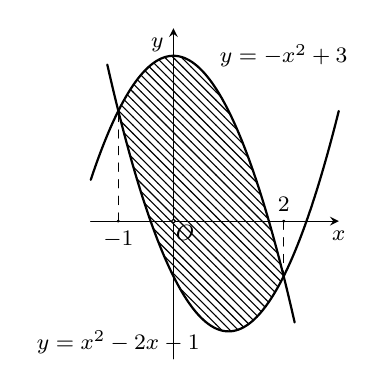
\begin{tikzpicture}[scale=.7, font=\footnotesize, line join=round, line cap=round, >=stealth]
			\draw[->] (-1.5,0) -- (3,0)node[below]{\footnotesize $x$};
			\draw (-1,0) circle (.5pt)node[below]{\footnotesize $-1$};
			\draw (2,0) circle (.5pt)node[above]{\footnotesize $2$};
			\draw[->,color=black] (0,-2.5) -- (0,3.5)node[below left]{\footnotesize $y$};
			\fill[pattern=north west lines] plot[smooth,samples=100,domain=-1:2] (\x,{(\x)^2-2*(\x)-1})--plot[smooth,samples=100,domain=2:-1] (\x,{-(\x)^2+3});
			\draw[thick,smooth,samples=100,domain=-1.5:2.2] plot(\x,{-(\x)^2+3});
			\draw[thick,smooth,samples=100,domain=-1.2:3] plot(\x,{(\x)^2-2*(\x)-1});
			\draw[dashed] (2,0) -- (2,-1) (-1,0) -- (-1,2);
			\filldraw[fill=white] (0,0) circle (1pt)node[shift={(-45:6pt)}]{\footnotesize $O$};
			\draw (2,3) node{\footnotesize $y=-x^2+3$};
			\draw (-1,-2.2) node{\footnotesize $y=x^2-2x-1$};
	\end{tikzpicture}}
	\loigiai{
		$S=\displaystyle\int\limits_{-1}^2\left[\left(-x^2+3\right)-\left(x^2-2x-1\right)\right]\mathrm{\,d}x=\displaystyle\int\limits_{-1}^2\left(-2x^2+2x+4\right)\mathrm{\,d}x$.
	}
\end{ex}
\begin{ex}%[Nguyễn Tuấn, dự án sáng tác đề 12]%[2D4H3-3]
	Thể tích của vật thể tròn xoay thu được khi quay hình phẳng (phần gạch sọc của hình vẽ) xung quanh trục $Ox$ bằng
\begin{center}
	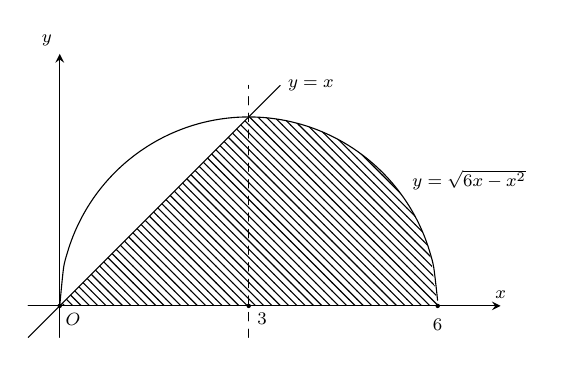
\begin{tikzpicture}[line join=round, line cap = round, >=stealth, scale=.8,font=\footnotesize,transform shape]
		\draw[->] (0,-.5)--(0,4) node[above left]{$y$};
		\draw[->] (-.5,0)--(7,0) node[above]{$x$};
		\def \f(#1){sqrt(6*#1 - #1*#1)};
		\draw[color=black,smooth,samples=100,domain=0:6] plot(\x,{\f(\x)});
		\draw 
		(6.5,2) node{$y=\sqrt{6x-x^2}$}
		(-.5,-.5)--(3.5,3.5) node[right]{$y=x$}
		;
		\draw[dashed](3,-.5)--(3,3.5);
		\fill[pattern=north west lines] plot[domain=3:6](\x,{\f(\x)})--(0,0)--cycle;
		\foreach \x/\y/\z/\g in {0/0/O/-45,3/0/3/-45,6/0/6/-90}
		\fill[black] (\x,\y) circle(1pt) ($(\x,\y)+(\g:3mm)$) node{$\z$};
	\end{tikzpicture}
\end{center}
	\choice
{$26\pi$}
{$25\pi$}
{\True $27\pi$}
{$24\pi$}
	\loigiai{
		\begin{center}
			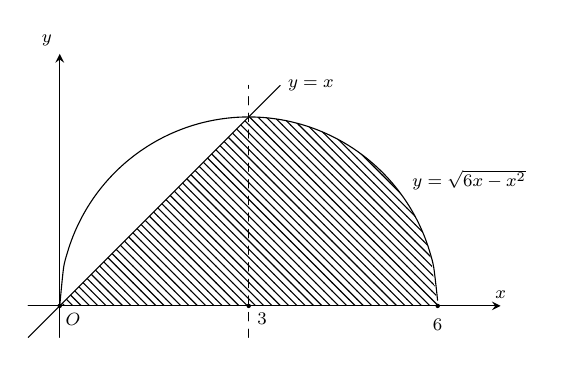
\begin{tikzpicture}[line join=round, line cap = round, >=stealth, scale=.8,font=\footnotesize,transform shape]
				\draw[->] (0,-.5)--(0,4) node[above left]{$y$};
				\draw[->] (-.5,0)--(7,0) node[above]{$x$};
				\def \f(#1){sqrt(6*#1 - #1*#1)};
				\draw[color=black,smooth,samples=100,domain=0:6] plot(\x,{\f(\x)});
				\draw 
				(6.5,2) node{$y=\sqrt{6x-x^2}$}
				(-.5,-.5)--(3.5,3.5) node[right]{$y=x$}
				;
				\draw[dashed](3,-.5)--(3,3.5);
				\fill[pattern=north west lines] plot[domain=3:6](\x,{\f(\x)})--(0,0)--cycle;
				\foreach \x/\y/\z/\g in {0/0/O/-45,3/0/3/-45,6/0/6/-90}
				\fill[black] (\x,\y) circle(1pt) ($(\x,\y)+(\g:3mm)$) node{$\z$};
			\end{tikzpicture}
		\end{center}
		Chia vật thể bởi mặt phẳng $x=3$ thì vật thể chia thành $2$ phần:
		\begin{itemize}
			\item Phần $1$ là khối tròn xoay khi quay hình phẳng giới hạn bởi các đường $y=x$, trục hoành và hai đường thẳng $x=0$, $x=3$ quanh trục $Ox$. Phần này có thể tích là:  
			$$V_1=\pi\displaystyle\int\limits_{0}^{3}x^2\mathrm{\,d}x=\pi\displaystyle\int\limits_{0}^{3}x^2\mathrm{\,d}x = \pi \dfrac{x^3}{3}\Big|_0^{3}=9\pi.$$
			\item Phần $2$ là khối tròn xoay khi quay hình phẳng giới hạn bởi các đường $y=\sqrt{6x-x^2}$, trục hoành và hai đường thẳng $x=3$, $x=6$ quanh trục $Ox$. Phần này có thể tích là:
			$$V_2=\pi\displaystyle\int\limits_{3}^{6}\left(\sqrt{6x - x^2} \right)^2\mathrm{\,d}x=\pi\displaystyle\int\limits_{3}^{6}\left(6x - x^2 \right)\mathrm{\,d}x = \pi\left( 3x^2 - \dfrac{x^3}{3} \right)\Big|_3^{6}=18\pi.$$
		\end{itemize}
		Vậy thể tích vật thể là $V=V_1+V_2=27\pi$.
	}
\end{ex}
\begin{ex}%[Nguyễn Tuấn, dự án sáng tác đề 12]%[2H5N1-2]
	Trong không gian $Oxyz$, cho mặt phẳng $(P)\colon 3x-z+2=0$. Véc-tơ nào dưới đây là một véc-tơ pháp tuyến của $(P)$?
	\choice
{$\overrightarrow{n}=\left(-1;0;-1\right)$}
{\True $\overrightarrow{n}=\left(3;0;-1\right)$}
{$\overrightarrow{n}=\left(3;-1;2\right)$}
{$\overrightarrow{n}=\left(3;-1;0\right)$}
	\loigiai{
		Mặt phẳng $(P)\colon 3x-z+2=0$ có một véc-tơ pháp tuyến là $\overrightarrow{n}=\left(3;0;-1\right)$.
	}
\end{ex}
\begin{ex}%[Nguyễn Tuấn, dự án sáng tác đề 12]%[2H5V2-3]
	Trong không gian $Oxyz$, cho điểm $A(1 ; 3 ; 2)$, mặt phẳng $(P)\colon 2 x-y+z-10=0$  và đường thẳng  $d\colon \dfrac{x+2}{2}=\dfrac{y-1}{1}=\dfrac{z-1}{-1}$. Đường thẳng $\Delta$ cắt $(P)$ và $d$ lần lượt tại hai điểm $M, N$ sao cho $A$ là trung điểm của đoạn $MN$. Biết rằng $\vec{u}=(a ; b ; 1)$ là một vectơ chỉ phương của $\Delta$, giá trị của $a+b$ bằng
	\choice
{\True $-11$}
{$3$}
{$11$}
{$-3$}
	\loigiai{
		Vì $N\in d$ nên $N\left(-2+2t;1+t;1-t \right)$ $t\in\mathbb{R}$. \\ Mặt khác, $A$ là trung điểm đoạn $MN$ nên $M(4-2t;5-t;3+t)$. \\
		Do $M \in (P)$ nên $2(4-2t)-(5-t)+3+t-10=0 \Leftrightarrow t = -2$. \\ Suy ra $M(8;7;1)$ và $N(-6;-1;3) \Rightarrow \vec{MN} =(-14;-8;2)$. \\
		Khi đó, đường thẳng $\Delta$ có một véc-tơ chỉ phương là  $\vec{u}=(-7 ; -4 ; 1)$. \\
		Suy ra $a = -7$ và $b = -4$. Vậy $a + b = -11$.
	}
\end{ex}
\begin{ex}%[Nguyễn Tuấn, dự án sáng tác đề 12]%[2H5H2-7]
	Trong không gian $Oxyz$, cô-sin của góc giữa đường thẳng chứa trục $Oy$ và mặt phẳng $(P)\colon 4x-3y+\sqrt{2}z-7=0$ bằng
	\choice
{$\dfrac{2}{\sqrt{3}}$}
{$\dfrac{1}{\sqrt{3}}$}
{$\dfrac{4}{\sqrt{3}}$}
{\True $\dfrac{\sqrt{2}}{\sqrt{3}}$}
	\loigiai{
		Véc-tơ chỉ phương của đường thẳng chứa trục $Oy$ là $\overrightarrow{j}=(0;1;0)$ và véc-tơ pháp tuyến của $(P)$ là $\overrightarrow{n}\left(4;-3;\sqrt{2}\right)$. Gọi $\alpha$ là góc giữa đường thẳng và mặt phẳng trên thì
		\[ \sin \alpha =\left| \cos \left(\overrightarrow{j},\overrightarrow{n}\right) \right| =\frac{1}{\sqrt{3}}. \]
		Suy ra $\cos \alpha =\sqrt{1-\sin^2\alpha}=\dfrac{\sqrt{2}}{\sqrt{3}}$.
	}
\end{ex}
\begin{ex}%[Nguyễn Tuấn, dự án sáng tác đề 12]%[2H5N3-2]
	Trong không gian $Oxyz$, mặt cầu $(S)\colon (x-1)^2+(y-2)^2+(z+3)^2=4$ có bán kính bằng
	\choice
{\True $2$}
{$4$}
{$16$}
{$\sqrt{2}$}
	\loigiai{Mặt cầu $(S)$ có bán kính $R=2$.}
\end{ex}
\begin{ex}%[Nguyễn Tuấn, dự án sáng tác đề 12]%[2D5H2-2]
	Cho $\mathrm{P}(A)=\dfrac{2}{5}$; $\mathrm{P}\left( B\mid A\right)=\dfrac{1}{3}$. Giá trị của $\mathrm{P}(AB)$ là 
	\choice
{$ \dfrac{1}{5}$}
{\True $\dfrac{2}{15} $}
{$ \dfrac{4}{15}$}
{$ \dfrac{3}{16}$}
	\loigiai{
		$\mathrm{P}(AB)=\mathrm{P}(A)\cdot \mathrm{P}\left( B\mid A\right)=\dfrac{2}{5}\cdot \dfrac{1}{3}=\dfrac{2}{15}$.
	}
\end{ex}
\begin{ex}%[Nguyễn Tuấn, dự án sáng tác đề 12]%[2D5V2-3]
	An có một túi gồm một số chiếc kẹo cùng loại, chỉ khác màu, trong đó có $6$ chiếc kẹo sô-cô-la đen, còn lại là $4$ chiếc kẹo sô-cô-la trắng. An lấy ngẫu nhiên $1$ chiếc kẹo trong túi để cho Bình, rồi lại lấy ngẫu nhiên tiếp 1 chiếc kẹo nữa trong túi và cũng đưa cho Bình. Xác suất để Bình nhận được $2$ chiếc kẹo sô-cô-la đen là 
	\choice
{$ \dfrac{3}{7}$}
{$ \dfrac{2}{5}$}
{$ \dfrac{1}{4}$}
{\True $\dfrac{1}{3} $}
	\loigiai{
		Gọi $A$ là biến cố: \lq\lq An lấy lần 1 được 1 chiếc kẹo sô-cô-la đen\rq\rq\, và $B$ là biến cố: \lq\lq An lấy lần 2 được 1 chiếc kẹo sô-cô-la đen\rq\rq.\\
		Khi đó $AB$ là biến cố: \lq\lq Cả hai lần đều lấy được kẹo sô-cô-la đen\rq\rq.\\
		Ta có $\mathrm{P}(A)=\dfrac{n(A)}{n(\Omega)}=\dfrac{6}{10}$.\\
		Sau khi lấy 1 chiếc kẹo sô-cô-la đen thì xác suất để chọn 1 chiếc kẹo sô-cô-la đen trong hộp đựng $5$ chiếc kẹo sô-cô-la đen, còn lại là $4$ chiếc kẹo sô-cô-la trắng là $\mathrm{P}(B\mid A)=\dfrac{5}{9}$.\\
		Khi đó $\mathrm{P}(AB)=\mathrm{P}(A)\cdot \mathrm{P}(B\mid A)=\dfrac{6}{10}\cdot \dfrac{5}{9}=\dfrac{1}{3}$.\\
		Xác suất để Bình nhận được $2$ chiếc kẹo sô-cô-la đen là $\dfrac{1}{3}$.
	}
\end{ex}
    \Closesolutionfile{ans}
    
    \subsection*{PHẦN II. Câu trắc nghiệm đúng sai. Thí sinh trả lời từ câu 1 đến câu 8. Trong mỗi ý a), b), c), d) ở mỗi câu, thí sinh chọn đúng hoặc sai.}
    \setcounter{ex}{0}
    \Opensolutionfile{ans}[ans-phanII]
    \begin{ex}%Cau1D %[2H5N3-3]
Cho $\left(S\right): x^2+y^2+z^2-2x-4y+6z-67=0$. Các mệnh đề sau đúng hay sai ?
\choiceTF
{\True Cho đường thẳng $\left(\Delta\right) :\heva{&x=1+t\\&y=2\\&z=-4+7t}$. Khi đó $\left(\Delta\right)$ và $\left(S\right)$ cắt nhau tại hai điểm}
{\True Bán kính mặt cầu $\left( S\right)$ là $R=9$}
{Cho mặt phẳng $\left(P\right): 2x-2y+z-13=0$. Khi đó $\left( P\right)$ tiếp xúc với $\left(S\right)$}
{Mặt cầu $\left( S\right)$ có tâm $I\left(1;2;3\right)$}
	\loigiai{
		\begin{itemchoice}
			\itemch Sai. Mặt cầu $\left( S\right)$ có tâm $I\left(1;2;-3\right)$.
			\itemch Đúng. Ta có $R=\sqrt{1^2+2^2+\left(-3\right)^2+67}=\sqrt{81}=9$
			\itemch Sai. Vì $\mathrm{d}\left(I,\left(P\right)\right)=\dfrac{\vert 2\cdot1-2\cdot2+\left(-3\right)-13\vert}{\sqrt{2^2+2^2+\left(-1\right)^2}}=6< R=9$. Suy ra $\left(P\right)$ cắt $\left(S\right)$ theo giao tuyến là một đường tròn.
			\itemch Đúng. Tọa độ giao điểm là nghiệm của hệ phương trình\\
	 $\heva{&x=1+t\\&y=2\\&z=-4+7t\\&x^2+y^2+z^2-2x-4y+6z-67=0}\Rightarrow  \hoac{&t=0\\&t=1}$.\\
	 Với $t=0$, thay $t=0$ vào $\left(\Delta\right)$ ta được tọa độ $A\left(1;2;-4\right)$\\
	 Với $t=1$, thay $t=1$ vào $\left(\Delta\right)$ ta được tọa độ $B\left(2;2;3\right)$.\\
	 Vậy, $\left(\Delta\right)$ và $\left(S\right)$ cắt nhau tại hai điểm $A$ và $B$.
		\end{itemchoice}
	}
\end{ex}
\begin{ex}%Cau2D %[2D5V1-2]
Trong một hộp có 20 viên bi xanh và 4 viên bi đỏ, các viên bi đều có hình dạng và kích thước giống nhau. Một học sinh lấy ngẫu nhiên lần lượt $2$ viên bi (lấy không hoàn lại) trong hộp.
Các khẳng định nào dưới đây đúng hay sai ? 
\choiceTF
{\True Xác suất để cả hai lần đều lấy được viên bi đỏ là $\dfrac{1}{46}$}
{\True Xác suất để ít nhất một lần lấy được viên bi xanh là $\dfrac{45}{46}$}
{\True Xác suất để lần thứ hai lấy được viên bi đỏ, biết lần thứ nhất lấy được viên bi đỏ, là $\dfrac{3}{23}$}
{Xác suất để lần thứ nhất lấy được viên bi đỏ là $\dfrac{1}{5}$}
	\loigiai{
		\begin{itemchoice}
			\itemch Sai. Xét biến cố:\\
	$A$:"Lần thứ nhất lấy được viên bi đỏ". Khi đó xác suất lần đầu lấy được viên bi đỏ là: $P(A)=\dfrac{4}{24}=\dfrac{1}{6}$.
			\itemch Đúng. Khi lần thứ nhất đã lấy được viên bi đỏ thì trong hộp còn $3$ viên bi đỏ. Gọi biến cố $B$: "Lần thứ hai lấy được viên bi đỏ", khi đó xác suất lần thứ hai lấy được viên bi đỏ khi biết lần thứ nhất lấy được viên bi đỏ là: $P(B \vert A)=\dfrac{3}{23}$
			\itemch Đúng. Xác suất để cả hai lần đều lấy được viên bi đỏ là: $P(C)=P(A \cap B)=P(A) \cdot P(B \vert A) = \dfrac{1}{6} \cdot \dfrac{3}{23}=\dfrac{1}{46}$. 
			\itemch Đúng. Xác suất để có ít nhất một lần lấy được viên bi xanh là:\\
			 $P(\overline{C})=1-P(C)= 1-\dfrac{1}{46}=\dfrac{45}{46}$. 
		\end{itemchoice}
	}
\end{ex}
\begin{ex}%Cau3D %[2H5H2-7]
	Trong không gian với hệ tọa độ $Oxyz$, cho mặt phẳng $(P)\colon 3x-y+2z+2=0$ và đường thẳng $d\colon\dfrac{x}{3}=\dfrac{y-1}{2}=\dfrac{z+1}{-1}$. Xác định tính đúng, sai của mỗi mệnh đề sau
	\choiceTF
{Góc giữa trục $Ox$ và $d$ (làm tròn đến hàng đơn vị của độ) bằng $42^\circ$}
{$(3;-1; -2)$ là véc-tơ pháp tuyến của $(P)$}
{\True Góc giữa $(P)$ và $(d)$ là $20^{\circ}$ (làm tròn đến hàng đơn vị của độ)}
{\True Góc giữa $(P)$ và $(d)$ là một góc nhọn}
	\loigiai{
	Ta có 	$\overrightarrow{n}_{(P)}=(1;-1; 2)$ là một véc-tơ pháp tuyến của $(P)$ và $\overrightarrow{u}_d=(1; 2;-1)$ là một véc-tơ chỉ phương của $d$.
		\begin{itemchoice}
		\itemch Sai. Ta có $\overrightarrow{n}_{(P)}=(3;-1; 2)$.
		\itemch Đúng. 
		$\sin\left(d,(P)\right)=\dfrac{\left|\overrightarrow{n}_{(P)}\cdot\overrightarrow{u}_d\right|}{\left|\overrightarrow{n}_{(P)}\right|\cdot\left|\overrightarrow{u}_d\right|} =\dfrac{|9-2-2|}{\sqrt{14}\cdot\sqrt{14}}=\dfrac{5}{14}$.  \\
		Suy ra 	$0<\sin\left(d,(P)\right)
e 1$ do đó góc giữa $(P)$ và $(d)$ là một góc nhọn.
			\itemch Sai. 
			Vậy $\sin\left(d,(P)\right)=\dfrac{\left|\overrightarrow{n}_{(P)}\cdot\overrightarrow{u}_d\right|}{\left|\overrightarrow{n}_{(P)}\right|\cdot\left|\overrightarrow{u}_d\right|} =\dfrac{|9-2-2|}{\sqrt{14}\cdot\sqrt{14}}=\dfrac{5}{14}\Rightarrow \left(d,(P)\right)\approx 21^{\circ}$.
			\itemch Sai.
			Ta có  $\overrightarrow{u}_{Ox}=\overrightarrow{i}=(1; 0;0)$.\\
			$\cos\left(d,Ox\right)=\dfrac{\left|\overrightarrow{u}_{d}\cdot\overrightarrow{i}\right|}{\left|\overrightarrow{u}_{d}\right|\cdot\left|\overrightarrow{i}\right|} =\dfrac{|3-0-0|}{\sqrt{14}\cdot\sqrt{1}}=\dfrac{3}{\sqrt{14}} \Rightarrow (d,Ox)\approx 37^{\circ}$.
			\end{itemchoice}}
\end{ex}
\begin{ex}%Cau4D %[2D5N2-4]
Xét một lô giày chiến sĩ được sản xuất bởi $3$ nhà máy $1$, $2$, $3$ với tỉ lệ lần lượt là $20\%$, $30\%$ và $50\%$. Xác suất giày hỏng của các nhà máy lần lượt là $0,001$; $0,005$ và $0,006$. Các khẳng định dưới đây đúng hay sai?
\choiceTF
{\True Lấy ngẫu nhiên một chiếc giày từ lô hàng. Xác suất để chiếc giày lấy ra là giày hỏng ở nhà máy $1$ là $0,002$ }
{Lấy ngẫu nhiên một chiếc giày từ lô hàng. Xác suất để chiếc giày lấy ra không bị hỏng là $0,9925$}
{\True Lấy ngẫu nhiên một chiếc giày từ lô hàng. Xác suất để chiếc giày lấy ra bị hỏng là $0,0065$}
{Lấy ngẫu nhiên ra một chiếc giày kiểm tra thì được kết quả là chiếc giày bị hỏng. Xác suất để chiếc giày đó do nhà máy $3$ sản xuất là $0,5$ (làm tròn đến chữ số thập phân thứ nhất)}
	\loigiai{ Gọi $A$: "lấy được giày hỏng", $A_i$:"lấy được giày ở nhà máy $i$" $\left(i=1,2,3\right)$. 
		\begin{itemchoice}
			\itemch Đúng. Ta có $P\left(A_1 \right)=0,2$, và $P\left(A \vert A_1 \right)=0,001$. Khi đó xác suất để chiếc giày lấy ra là giày hỏng ở nhà máy $1$ là $0,2 \cdot 0,001=0,002$.
			\itemch Đúng. Ta có $\left\lbrace A_1,A_2,A_3 \right\rbrace$ là hệ đầy đủ. Áp dụng công thức toàn phần ta có:
			\begin{eqnarray*}
&P\left(A\right) &= P\left(A_1\right)\cdot P\left(A\vert A_1 \right)+P\left(A_1\right)\cdot P\left(A\vert A_1 \right)+P\left(A_1\right)\cdot P\left(A\vert A_1 \right)\\
& &= 0,2 \cdot 0,001+0,3 \cdot 0,005+0,5 \cdot 0,006\\
& &= 0,0065
			\end{eqnarray*}
			\itemch Sai. Ta có $P\left(\overline{A}\right)=1-P\left(A\right)=1-0,0065=0,9935$.
			\itemch Sai. Ta có:$$P\left(A_3\vert A \right)=\dfrac{P\left(A_3\right)\cdot P\left(A \vert A_3\right)}{P\left(A\right)}=\dfrac{0,5\cdot 0,006}{0,0065}=\dfrac{6}{13}\approx 0,5$$
			Vậy xác suất để chiếc giày đó do nhà máy $3$ sản xuất là $0,5$.
		\end{itemchoice}
	}
\end{ex}

    \Closesolutionfile{ans}
    
    \subsection*{PHẦN III. Câu hỏi trả lời ngắn. Thí sinh trả lời từ câu 1 đến câu 6.}
    \setcounter{ex}{0}
    \Opensolutionfile{ans}[ans-phanIII]
    \begin{ex}%[Nguyễn Tuấn, dự án sáng tác đề 12]%[2H5H3-3]
	Trong không gian $Oxyz$, cho hai điểm $A(2;0;-1)$ và $B(0;2;3)$. Mặt cầu $(S)$ đường kính $AB$ có bán kính $R$. Khi đó $8R^2$ bằng
	\shortans{$48$}
	\loigiai{
		Gọi $I$ là trung điểm của $AB$.\\ 
		Khi đó, mặt cầu $(S)$ có tâm $I$ và bán kính $R=\dfrac{AB}{2}$.\\
		$\Rightarrow I(1;1;1)$, $R=\dfrac{1}{2} \sqrt{(0-2)^2+(2-0)^2+(3+1)^2}=\sqrt{6}$.\\
		Vậy $8R^2=48$.
	}
\end{ex}
\begin{ex}%[Nguyễn Tuấn, dự án sáng tác đề 12]%[2H5V2-2]
	Trong không gian $Oxyz$, cho điểm $M(1;0;2)$ và đường thẳng $d\colon \dfrac{x}{2}=\dfrac{y-1}{-1}=\dfrac{z-3}{1}$. Đường thẳng $\Delta$ đi qua $M$ cắt và vuông góc với $d$ có một véc-tơ chỉ phương là $\overrightarrow{u}=(a;b;4)$. Giá trị biểu thức $S=a+b$ bằng
	\shortans{$1$}
	\loigiai{
		Giả sử $H$ là giao điểm của hai đường thẳng $\Delta$ và $d$. Khi đó $H(2t;1-t;3+t)$.\\
		Vì $\Delta\perp d$ nên $\overrightarrow{MH}\cdot \overrightarrow{u}_d=0$.\\
		Ta có $\overrightarrow{MH}=(2t-1;1-t;1+t)$, $\overrightarrow{u}_d=(2;-1;1)$, suy ra
		$$2\cdot (2t-1)-1\cdot (1-t)+1\cdot (1+t)=0\Leftrightarrow t=\dfrac{1}{3}.$$
		Suy ra $\overrightarrow{MH}=\left(-\dfrac{1}{3};\dfrac{2}{3};\dfrac{4}{3}\right)$, vậy $\overrightarrow{u}=(-1;2;4)$ cũng là véc-tơ chỉ phương của $\Delta$.\\
		Vậy $a=-1$, $b=2$ hay $a+b=1$.
	}
\end{ex}
\begin{ex}%[Nguyễn Tuấn, dự án sáng tác đề 12]%[2D5V2-3] 
	Chuồng I có 5 con gà mái, 2 con gà trống. Chuồng II có 3 con gà mái, 5 con gà trống. Bác Mai bắt một con gà trong số đó theo cách sau: Bác tung một con xúc xắc cân đối, đồng chất. Nếu số chấm chia hết cho 3 thì bác chọn chuồng I, nếu số chấm không chia hết cho 3 thì bác chọn chuồng II. Sau đó, từ chuồng đã chọn bác bắt ngẫu nhiên một con gà. Gọi $P$ là xác suất để bác Mai bắt được con gà mái. Khi đó $84P$ bằng
	\shortans{$41$}
	\loigiai{
		Gọi $A$ là biến cố: \lq\lq Bác Mai bắt được con gà mái\rq\rq.\\
		Gọi $B_1$ là biến cố: \lq\lq tung con xúc xắc được số chấm chia hết cho $3$\rq\rq\, suy ra $\mathrm{P}(B_1)=\dfrac{2}{6}=\dfrac{1}{3}$.\\
		Gọi $B_2$ là biến cố: \lq\lq tung con xúc xắc được số chấm không chia hết cho $3$\rq\rq\, suy ra $\mathrm{P}(B_2)=\dfrac{4}{6}=\dfrac{2}{3}$.\\
		Ta có  xác suất bắt được gà mái từ chuồng I là $\mathrm{P}\left(A\mid B_1\right)=\dfrac{5}{7}$.\\
		Ta có  xác suất bắt được gà mái từ chuồng II là $\mathrm{P}\left(A\mid B_2\right)=\dfrac{3}{8}$.\\
		Áp dụng công thức xác suất toàn phần ta có
		$$\mathrm{P}(A)=\mathrm{P}(B_1)\cdot \mathrm{P}(A\mid B_1)+\mathrm{P}(B_2)\cdot \mathrm{P}(A\mid B_2)=\dfrac{1}{3}\cdot \dfrac{5}{7}+\dfrac{2}{3}\cdot \dfrac{3}{8}=\dfrac{41}{84}.$$
		Vậy xác suất để bác Mai bắt được con gà mái là $\dfrac{41}{84}$.\\
		Vậy $84P=41$.
	}
\end{ex}
\begin{ex}%[Nguyễn Tuấn, dự án sáng tác đề 12]%[2D4H3-3]
	\immini
	{
		Một vật trang trí có dạng khối tròn xoay tạo thành khi quay miền $(R)$ được giới hạn bởi đường gấp khúc $DABFE$ và cung tròn $ED$ (phần gạch chéo trong hình bên) xung quanh trục $AB$. Biết $ABCD$ là hình chữ nhật cạnh $AB =3$ cm, $AD=2$ cm; $F$ là trung điểm của $BC$; điểm $E$ cách $AD$ một đoạn bằng $1$ cm. Tính thể tích của vật trang trí đó, làm tròn kết quả đến hàng phần mười, đơn vị cm$^3$.
		\shortans{$16{,}5$}
	}
	{
		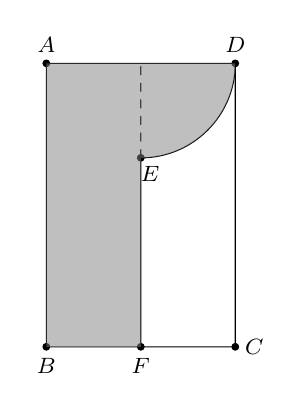
\begin{tikzpicture}[scale=1.2, line join=round, line cap=round,>=stealth,font=\footnotesize]
			\path (0,0) coordinate (B)	(2,0) coordinate (C) (2,3) coordinate (D) (0,3) coordinate (A) ($(B)!.5!(C)$) coordinate (F) ($(F)+(0,2)$) coordinate (E) ($(A)!.5!(D)$) coordinate (I) ;
			\draw (A)--(B)--(C)--(D)--cycle (E)--(F);
			\draw[dashed] (E)--(I);
			\foreach \d/\g in {A/90,B/-90,C/0,D/90,F/-90,E/-60}
			\draw[fill=black] (\d) circle (1pt) +(\g:0.2) node{$\d$};
			\draw (E) arc (-90:0:1cm); 
			\fill[color=gray,opacity=0.5] (A)--(B)--(F)--(I)--cycle (E) arc (-90:0:1cm)--(D)--(I)--cycle;
		\end{tikzpicture}
	}
	\loigiai{
		\immini
		{
			Gắn hệ trục tọa độ như hình vẽ bên.\\
			Quay hình chữ nhật $GEFB$ xung quanh trục $AB$ ta được khối trụ có bán kính đáy bằng $1$ và chiều cao bằng $2$.\\
			Phương trình đường tròn tâm $I$ bán kính bằng $1$ là $x^2+(y-1)^2=1$, suy ra phương trình của cung $DE$ là $y=1+\sqrt{1-x^2}$.\\
			Vây thể tích của vật trang trí là
			$$V=\pi \displaystyle\int\limits_{0}^{1} \left(1+\sqrt{1-x^2}\right)^2 \mathrm{\,d}x+\pi \cdot 1^2\cdot 2\approx 16{,}5\ (\mathrm{cm}^3).$$
		}
		{
			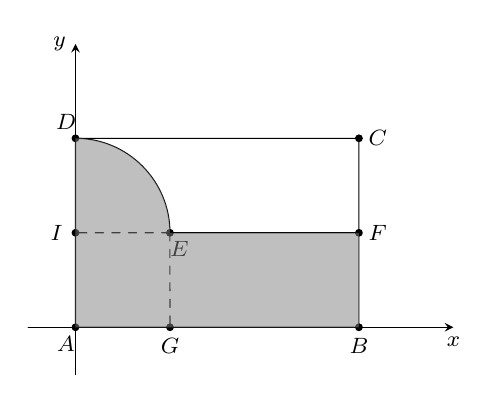
\begin{tikzpicture}[scale=1.2, line join=round, line cap=round,>=stealth,font=\footnotesize]
				\draw[->] (-0.5,0)--(4,0) node[below]{$x$};
				\draw[->] (0,-0.5)--(0,3) node[left]{$y$};
				\path (0,0) coordinate (A)	(3,0) coordinate (B) (3,2) coordinate (C) (0,2) coordinate (D) ($(B)!.5!(C)$) coordinate (F) ($(F)-(2,0)$) coordinate (E) ($(A)!.5!(D)$) coordinate (I) (1,0) coordinate (G) ;
				\draw (A)--(B)--(C)--(D)--cycle (E)--(F);
				\draw[dashed] (E)--(I) (E)--(G);
				\foreach \d/\g in {A/-120,B/-90,C/0,D/120,F/0,E/-60,I/180,G/-90}
				\draw[fill=black] (\d) circle (1pt) +(\g:0.2) node{$\d$};
				\draw (E) arc (0:90:1cm); 
				\fill[color=gray,opacity=0.5] (A)--(B)--(F)--(I)--cycle (E) arc (0:90:1cm)--(D)--(I)--cycle;
			\end{tikzpicture}	
		}
	}
\end{ex}
\begin{ex}%[Nguyễn Tuấn, dự án sáng tác đề 12]%[2D4C3-1]
	Cho hàm số bậc bốn $y=f(x)$ có ba điểm cực trị dương lần lượt là $x_1$, $x_2$, $x_3$ thỏa mãn $x_1+x_2+x_3=3$ và $g(x)$ là parabol đi qua ba điểm cực trị của đồ thị hàm số $f(x)$. Diện tích hình phẳng giới hạn bởi đồ thị của hàm số $y=\dfrac{f'(x)}{f(x)-g(x)}$, trục hoành và hai đường thẳng $x=-2$, $x=0$ bằng (kết quả làm tròn đến hàng phần trăm).
	\shortans{$4{,}39$}
	\loigiai{
		Giả sử $f(x)=ax^4+bx^3+cx^2+dx+e$ với $a$, $b$, $c$, $d$, $e\in\mathbb{R}$.\\
		Ta có $f'(x)=4ax^3+3bx^2+2cx+d=4a(x-x_1)(x-x_2)(x-x_3)$.\\
		Mà theo Định lý Vi-ét ta có $x_1+x_2+x_3=3\Leftrightarrow -\dfrac{3b}{4a}=3$.\\
		Vì $g(x)$ là hàm số bậc hai đi qua $3$ điểm cực trị của đồ thị $f(x)$ nên phương trình $f(x)=g(x)$ nhận $x_1$, $x_2$, $x_3$ là nghiệm. Vậy
		$$f(x)-g(x)=ax^4+bx^3+\left(cx^2+dx+e-g(x)\right)=a(x-x_1)(x-x_2)(x-x_3)(x-x_4).$$
		Ta có $x_1+x_2+x_3+x_4=-\dfrac{b}{a}=4$ mà $x_1+x_2+x_3=3$ nên $x_4=1$.\\
		Vậy $\dfrac{f'(x)}{f(x)-g(x)}=\dfrac{4}{x-1}$. Suy ra
		$$S=\displaystyle\int\limits_{-2}^{0} \left|\dfrac{4}{x-1}\right| \mathrm{\,d}x=4\ln 3\approx 4{,}39.$$
	}
\end{ex}
\begin{ex}%[Nguyễn Tuấn, dự án sáng tác đề 12]%[2H5C3-3]
	Trong không gian với hệ tọa độ $Oxyz$ cho điểm $A(-2;2;-2)$ và điểm $B(3;-3;3)$. Điểm $M$ thay đổi trong không gian thỏa mãn $\dfrac{MA}{MB}=\dfrac{2}{3}$. Điểm $N(a;b;c)$ thuộc mặt phẳng $(P)\colon-x+2y-2z+6=0$ sao cho $MN$ nhỏ nhất. Tính tổng $T=a+b+c$.
\shortans{$-2$}
	\loigiai{
		\immini
		{
			Gọi $M(x;y;z)$, ta có $\overrightarrow{MA}=(-2-x;2-y;-2-z)$,\\ $\overrightarrow{MB}=(3-x;-3-y;3-z)$. Vậy $$\dfrac{MA}{MB}=\dfrac{2}{3} \Leftrightarrow 9MA^2=4MB^2 \Leftrightarrow (x+6)^2+(y-6)^2+(z+6)^2=108.$$
			Vậy điểm $M$ thuộc mặt cầu tâm $I(-6;6 ;-6)$ bán kính $R=6\sqrt{3}$.\\
			Vậy $MN$ nhỏ nhất khi $M, N$ thuộc đường thẳng đi qua tâm $I$ và vuông góc với mặt phẳng $(P)$.\\
			Gọi $(d)$ là đường thẳng đi qua tâm $I$ và vuông góc với mặt phẳng $(P)$. Ta được $(d)\colon \heva{&x=-6-t \\& y=6+2t \\& z=-6-2t}$.\\
			Tọa độ điểm $N$ là nghiệm của hệ phương trình
			$$
			\begin{aligned}
				&\heva{& {x=-6-t} \\& {y=6+2t} \\& {z=-6-2t} \\& {-x+2y-2z+6=0}} \Leftrightarrow \heva{& {x=-6-t} \\& {y=6+2t} \\& {z=-6-2t} \\& {6+t+12+4t+12+4t+6=0}} \Leftrightarrow \heva{& x=-2 \\& y=-2 \\& z=2 \\& t=-4.}
			\end{aligned}
			$$
			Suy $N(-2;-2;2)$ nên ta được $T=-2-2+2=-2$.
		}
		{
			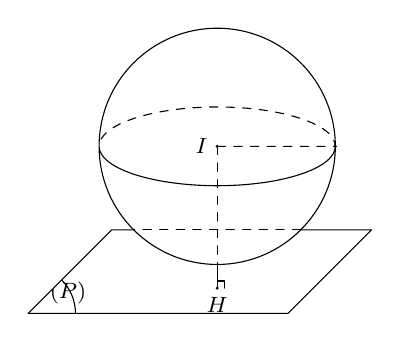
\begin{tikzpicture}[scale=.6, font=\footnotesize, line join=round, line cap=round, >=stealth]
				\def\R{2.5} 
				\def\t{.15} 
				\coordinate[label=left:$I$] (O) at (0,0);
				\coordinate (A) at (\R,0);
				\draw (O) circle (\R) (A) arc (0:-180: {\R} and {\R/3});
				\draw[dashed] (O)--(A) arc (0:180: {\R} and {\R/3});
				\foreach \diem in {A,O}	\fill (\diem)circle(1pt);
				\coordinate (M) at ($(0,0)+(-45:\R cm)$);
				\coordinate (N) at ($(0,0)+(-135:\R cm)$);
				\draw[dashed] (M)--(N);
				\draw (M)--++(0:1.5)--++(-135:2.5)coordinate (I)--++(180:5.5)coordinate (J) --++(45:2.5)coordinate (K)--(N);
				\draw[dashed] (O)--++(-90:\R)--++(-90:0.5)coordinate (H);
				\draw (H)--++(90:0.5);
				\fill (H) circle (1pt) node[below]{$H$};
				\def\t{.15}
				\draw (H)--++(90:\t)--++(0:\t)--++(-90:\t);
				\clip (I) -- (J) -- (K);
				\draw (J) circle (1cm);
				\draw ($(J)+(0.25,0)$) node[above right]{$(P)$};
			\end{tikzpicture}
			
		}
		
	}
\end{ex}
    \Closesolutionfile{ans}
    
    \hetde\label{\made}
    \newpage
    \begin{center}
    \textbf{\large BẢNG ĐÁP ÁN}
    \end{center}
    \noindent\textbf{A. ĐÁP ÁN PHẦN I}
    \inputansbox{10}{ans-phanI}
    \noindent\textbf{B. ĐÁP ÁN PHẦN II}
    \inputansbox[2]{2}{ans-phanII}
    \noindent\textbf{C. ĐÁP ÁN PHẦN III}
    \inputansbox[3]{6}{ans-phanIII}

\vspace*{1cm}
\begin{flushright}
\begin{minipage}{0.8\textwidth}
    \begin{center}
        TP. Hồ Chí Minh, ngày 20 tháng 5 năm 2025\\[.5cm]
        \textbf{Ký Tên}\\[3cm]
        \textbf{Nguyễn Văn Sang}
    \end{center}
\end{minipage}
\end{flushright}
\end{document}
    